\documentclass[a4paper,14pt]{extarticle}

\usepackage[a4paper,top=20mm,bottom=20mm,left=30mm,right=10mm]{geometry}
\usepackage[T1,T2A]{fontenc}
\usepackage[utf8]{inputenc}
\usepackage[russian]{babel}
\usepackage{indentfirst}
\usepackage{titlesec}
\usepackage{graphicx}
\usepackage{verbatim}
\usepackage{fancyvrb}

\renewcommand{\baselinestretch}{1.3}
\titleformat{\section}{\normalsize\bfseries}{\thesection}{1em}{}
\titleformat{\subsection}{\normalsize\bfseries}{\thesection}{1em}{}
\setlength{\parindent}{12.5mm}

\begin{document}

  \newpage\thispagestyle{empty}
  \begin{center}
    \MakeUppercase{
      Министерство науки и высшего образования Российской Федерации\\
      Федеральное государственное бюджетное образовательное учреждение высшего образования\\
      <<Вятский Государственный Университет>>\\
    }
    Институт математики и информационных систем\\
    Факультет автоматики и вычислительной техники\\
    Кафедра электронных вычислительных машин
  \end{center}
  \vfill

  \begin{center}
    Отчет по лабораторной работе №7\\
    по дисциплине\\
    <<Программирование>>\\
  \end{center}
  \vfill

  \noindent
  \begin{tabular}{ll}
    Выполнил студент гр. ИВТб-1301-05-00 \hspace{5mm} &
    \rule[-1mm]{25mm}{0.10mm}\,/Макаров С.А./\\
    
    Руководитель зав. кафедры ЭВМ & \rule[-1mm]{25mm}{0.10mm}\,/Долженкова М.Л./\\
  \end{tabular}

  \vfill
  \begin{center}
    Киров 2025
  \end{center}

  \newpage
  \section*{Цель}
  Цель лабораторной работы: получение навыков реализации алгоритмов с рекурсивными вычислениями, знакомство с фракталами.

  \section*{Задание}
  \begin{enumerate}
    \item Написать программу для визуализации фрактала <<Кривая Хартера-Хейтуэя>>.
    \item Предусмотреть возможности масштабирования, изменения глубины прорисовки и перемещения полученной фигуры.
    \item Построение множества ломанных, образующих фрактал, должно осуществляться в отдельном модуле.
  \end{enumerate}

  \pagebreak
  \section*{Решение}

  \begin{figure}[h]
    \centering
    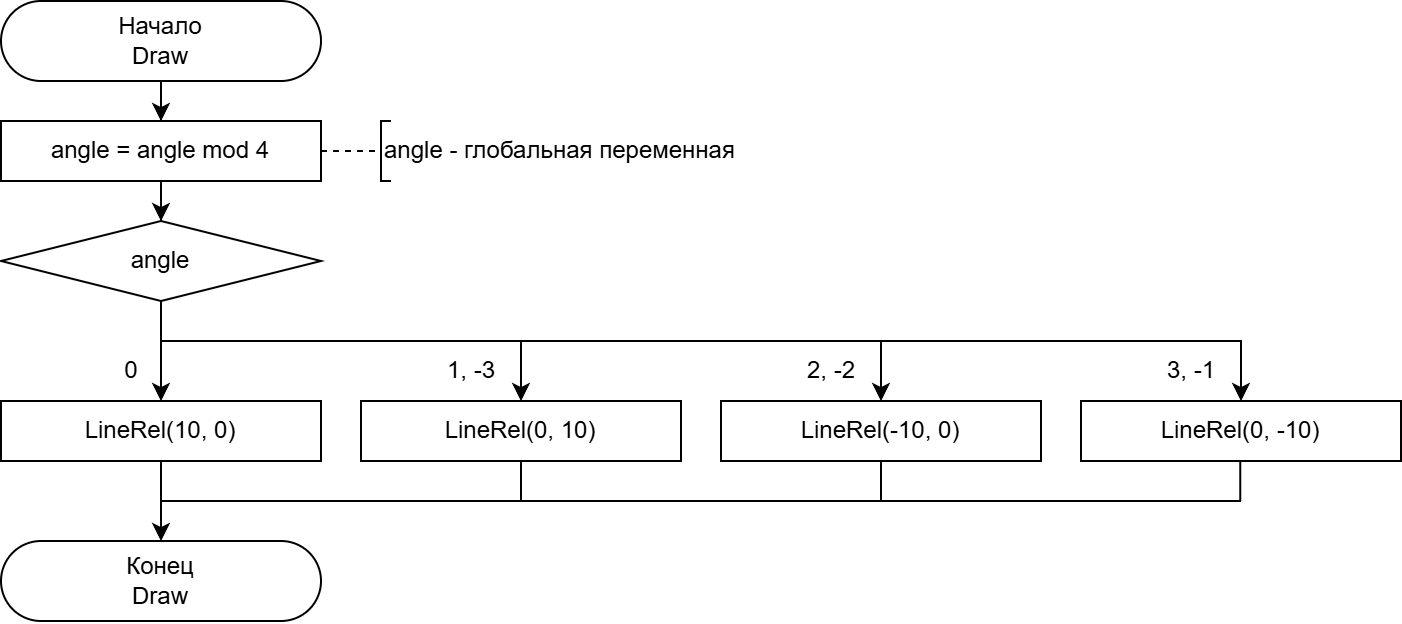
\includegraphics[width=1\linewidth]{images/s-1}
  \end{figure}
  \begin{center}
    Рисунок 1 – Схема алгоритма отрисовки отрезка
  \end{center}

  \begin{figure}[h]
    \centering
    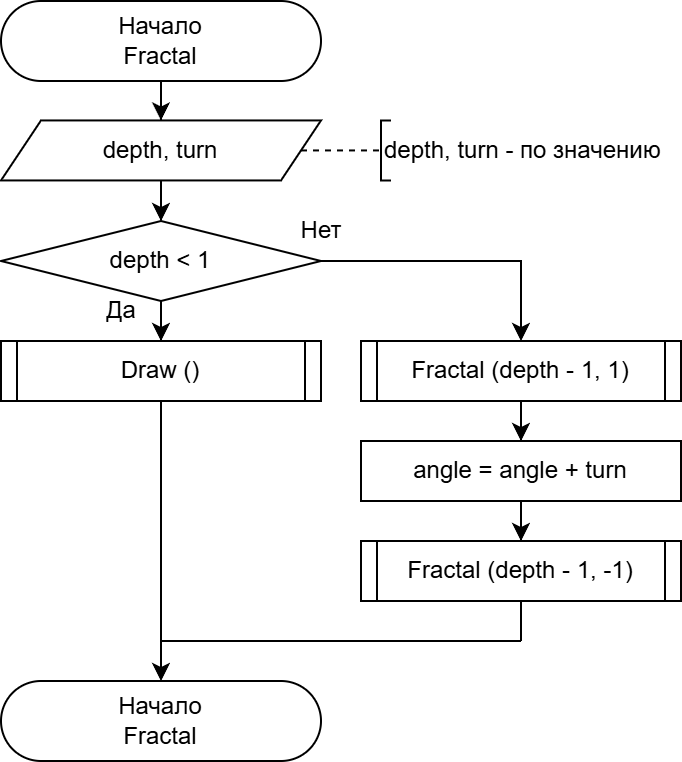
\includegraphics[width=0.5\linewidth]{images/s-2}
  \end{figure}
  \begin{center}
    Рисунок 2 – Схема алгоритма построения кривой
  \end{center}

  \pagebreak

  \begin{figure}[h]
    \centering
    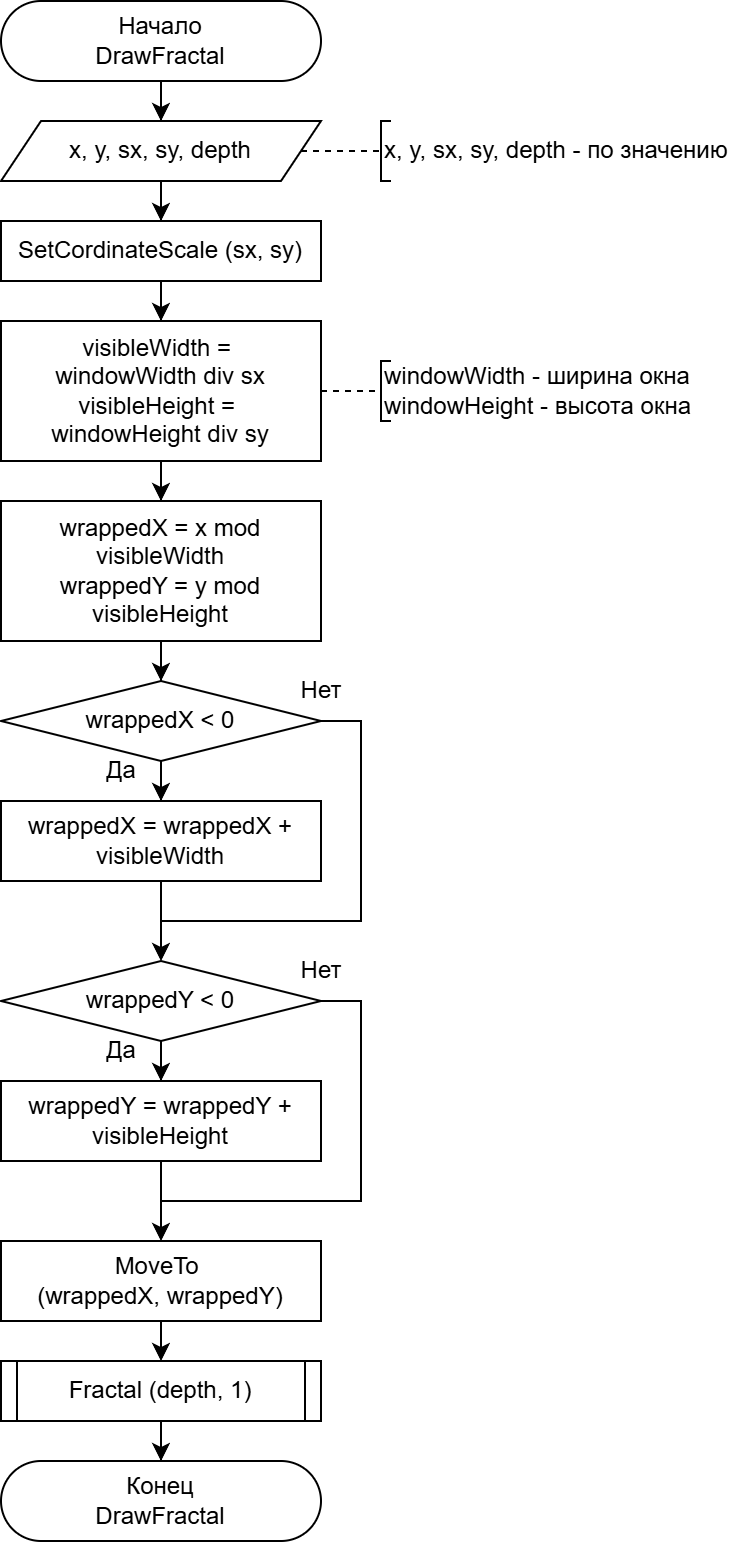
\includegraphics[width=0.55\linewidth]{images/s-3}
  \end{figure}
  \begin{center}
    Рисунок 3 – Схема алгоритма построения фрактала
  \end{center}

  \pagebreak

  \begin{figure}[h]
    \centering
    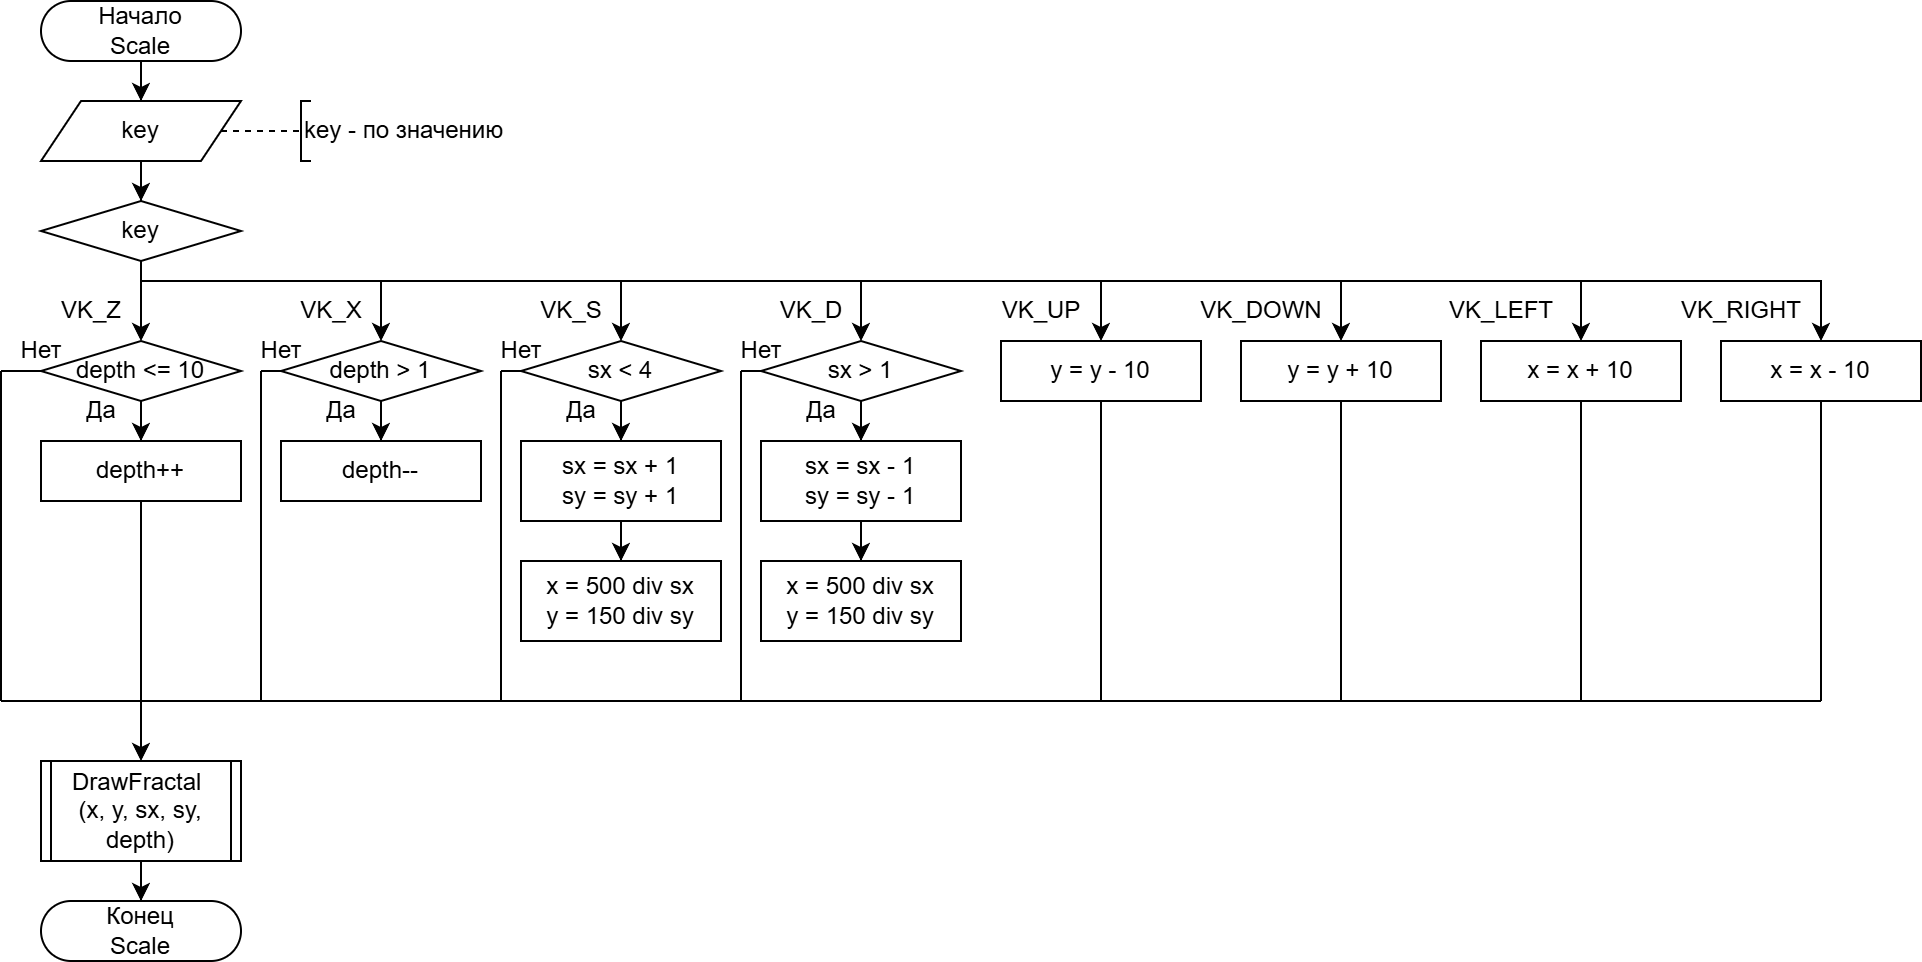
\includegraphics[width=1\linewidth]{images/s-4}
  \end{figure}
  \begin{center}
    Рисунок 4 – Схема алгоритма обработки клавиш
  \end{center}

  \begin{figure}[h]
    \centering
    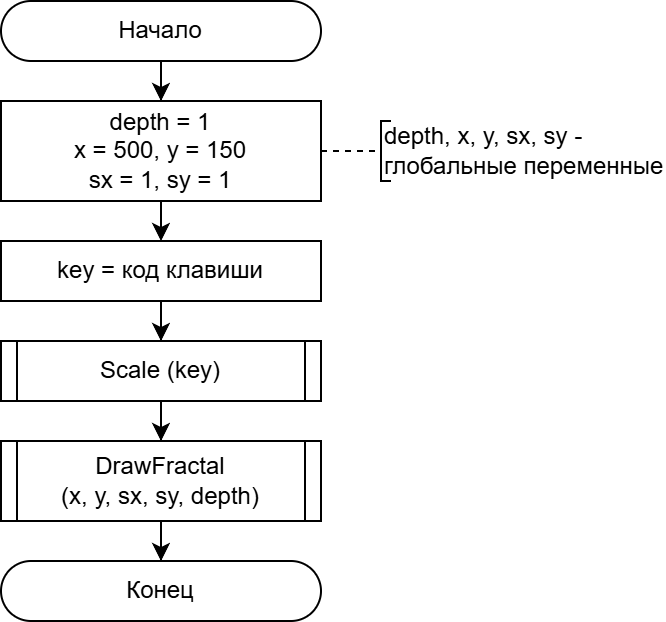
\includegraphics[width=0.5\linewidth]{images/s-5}
  \end{figure}
  \begin{center}
    Рисунок 5 – Схема алгоритма программы
  \end{center}

  \pagebreak

  Исходный код модуля для построения множества ломанных:

  \noindent
  \begin{Verbatim}[tabsize=4,fontsize=\small]
unit Dragon;
interface
uses
  GraphABC;
procedure DrawFractal(x, y, sx, sy, depth: integer);
implementation
  var
    angle: integer;
  procedure Draw();
  begin
    angle := angle mod 4;
    case angle of
      0: LineRel(10, 0);
      1, -3: LineRel(0, 10);
      2, -2: LineRel(-10, 0);
      3, -1: LineRel(0, -10);
    end;
  end;
  procedure Fractal(depth, turn: integer);
  begin
    if depth < 1 then
    begin
      Draw();
      exit;
    end;
    Fractal(depth - 1, 1);
    angle := angle + turn;
    Fractal(depth - 1, -1);
  end;
  procedure DrawFractal(x, y, sx, sy, depth: integer);
  var
    wrappedX, wrappedY: integer;
    visibleWidth, visibleHeight: integer;
  begin
    SetCoordinateScale(sx, sy);
    visibleWidth := WindowWidth div sx;
    visibleHeight := WindowHeight div sy;
    wrappedX := x mod visibleWidth;
    wrappedY := y mod visibleHeight;
    if wrappedX < 0 then wrappedX := wrappedX + visibleWidth;
    if wrappedY < 0 then wrappedY := wrappedY + visibleHeight;
    MoveTo(wrappedX, wrappedY);
    angle := 0;
    Fractal(depth, 1);
  end;
end.
  \end{Verbatim}

  Исходный код основного модуля представлен ниже:

  \noindent
  \begin{Verbatim}[tabsize=4,fontsize=\small]
uses
  GraphABC, Dragon;
var
  depth: integer = 1;
  x: integer = 500;
  y: integer = 150;
  sx: integer = 1;
  sy: integer = 1;
procedure Scale(key: integer);
begin
  case key of
    VK_Z:
      begin
        if depth <= 10 then 
          depth += 1 
        else
          exit;
      end;
    VK_X:
      begin
        if depth > 1 then
          depth -= 1
        else
          exit;
      end;
    VK_S:
      if sx < 4 then
      begin
        sx := sx + 1;
        sy := sy + 1;
        x := 500 div sx; y := 150 div sy;
      end;
    VK_D:
      if sx > 1 then
      begin
        sx := sx - 1;
        sy := sy - 1;
        x := 500 div sx; y := 150 div sy;
      end;
    VK_UP:
      y := y - 10;
    VK_DOWN:
      y := y + 10;
    VK_LEFT:
      x := x - 10;
    VK_RIGHT:
      x := x + 10;
  end;
  Window.Clear();
  DrawFractal(x, y, sx, sy, depth);
end;
begin
  SetWindowSize(800, 600);
  OnKeyDown := Scale;
  DrawFractal(x, y, sx, sy, depth);
end.
  \end{Verbatim}

  \section*{Вывод}
  В ходе выполнения лабораторной работы получены навыки реализации алгоритма с рекурсивным вычислением, а также был построен фрактал <<Кривая Хартера-Хейтуэя>>.

\end{document}